\section{Architektur}
Nun gilt es das in Kapitel \ref{sec:konzept} vorgestellte Konzept umzusetzen. Dazu haben wir eine Architektur für einen Sprachassistenten entwickelten, welche in Abbildung \ref{fig:infrastruktur-overview} zu sehen ist. Diese Architektur soll mehr Privatsphäre bieten und unterteilt sich in drei Hauptmodul: die mobile App, das Repository und die Cloud. Was auffällt, das es zweimal das Untermodul "Speech Processing" gibt. Dabei wird in der mobilen App einfache Sprachverarbeitung wie beispielsweise das Aufnehmen bzw. die Wiedergabe eines Audiofiles implementiert. Ressourcen intensive Sprachverarbeitungsprozesse wie beispielsweise die Umwandlung von Sprache zu Text werden in die Cloud ausgelagert. Im folgenden werden die drei Hauptmodule genauer beschrieben.
\begin{figure}[h!]
	\centering
	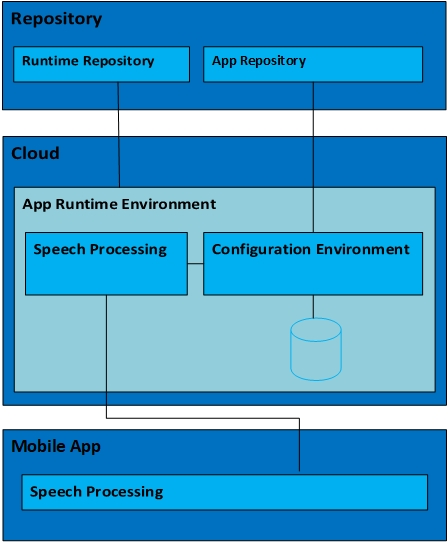
\includegraphics[width=0.7\linewidth]{Picture/Infrastruktur-Overview.jpg}
	\caption[Architektur Übersicht]{Architektur Übersicht}
	\label{fig:infrastruktur-overview}
\end{figure}

\subsection{Mobile App}
Die mobile App ist die Schnittstelle zum Nutzer und wie Abbildung \ref{fig:infrastruktur-app} zeigt, hat diese drei Module:

\begin{itemize}
	\item \textsl{Speech Recording:} Aufnehmen und streamen der Eingabe eines Nutzers an die Cloud.
	\item \textsl{Speech Playback:} Abspielen eines Streams, der von der Cloud erzeugt wurde.
	\item \textsl{Hotword Detection:} Die mobile App soll nicht ununterbrochen die Eingabe des Nutzers aufnehmen und streamen, denn diese könnte die Privatsphäre des Nutzer beeinträchtigen. Die App soll nur aufnehmen und streamen, wenn der Nutzer das will. Somit kommt die sogenannte "Hotword Detection" zum Einsatz. Dies belauscht den Nutzer durchgängig, jedoch nur lokal auf dem Endgerät und ohne Daten via Internetverbindung weiter zu senden. Eine Hotword Detection benötigt kaum Ressourcen, da sie für die Erkennung eines einzigen Signalwortes optimiert wurde. Somit lässt sich ein Signalwort definieren, sobald der Nutzer dieses Signalwort sagt, wird das Aufnehmen und streamen an die Cloud gestartet.
\end{itemize}

\begin{figure}[h!]
	\centering
	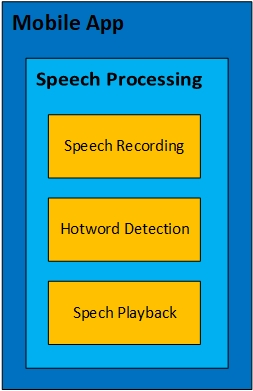
\includegraphics[width=0.3\linewidth]{Picture/Infrastruktur-App.jpg}
	\caption[Architektur - mobile App]{Architektur - mobile App}
	\label{fig:infrastruktur-app}
\end{figure}

\subsection{Repository}
Das Repository ist in Abbildung \ref{fig:infrastruktur-repository} dargestellt und unterteilt sich nochmals in zwei Module: das Runtime Repository und das App Repository, welche im folgenden genauer beschrieben werden.

\begin{itemize}
	\item \textsl{Runtime Repository:} Das Runtime Repository stellt eine Laufzeitumgebungen für die Cloud bereit. Die Laufzeitumgebung beinhaltet das Betriebssystem und alle vom Sprachassistenten benötigten Pakete und wird in verschieden Formaten bereitgestellt. Ein Nutzer kann sich eine Laufzeitumgebung im Format seiner Wahl herunterladen und auf seiner privaten Cloud installieren. Dabei soll die Installation möglichst wenig Konfigurationsaufwand mit sich bringen, denn auch Nutzer ohne IT-Background sollen sich diese Umgebungen installieren können. 
	\item \textsl{App Repository:} Das App Repository stellt alle Apps bereit, die auf dem Sprachassistenten genutzt werden können. Will ein Nutzer ein App nutzen, so muss er diese in seiner Laufzeitumgebung installieren.
\end{itemize}


\begin{figure}[h!]
	\centering
	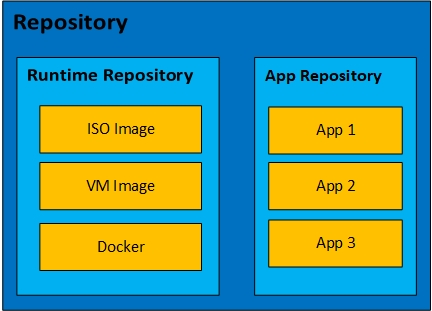
\includegraphics[width=0.6\linewidth]{Picture/Infrastruktur-Repository.jpg}
	\caption[Architektur - mobile App]{Architektur - Repository}
	\label{fig:infrastruktur-repository}
\end{figure}

\subsection{Laufzeitumgebung}
Die Laufzeitumgebung ist das Herzstück des Sprachassistenten und ist in Abbildung \ref{fig:infrastruktur-cloud} aufgezeigt. Sie beinhaltet die meisten Module sowie Funktionen.

\begin{figure}[h!]
	\centering
	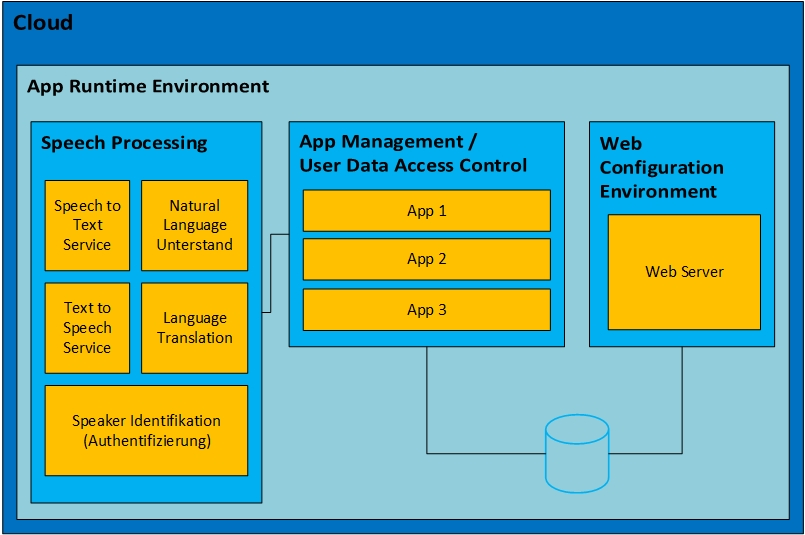
\includegraphics[width=0.9\linewidth]{Picture/Infrastruktur-Cloud.jpg}
	\caption[Architektur - mobile App]{Architektur - Cloud}
	\label{fig:infrastruktur-cloud}
\end{figure}

\begin{itemize}
	\item \textsl{Speech Processing:} Das Modul Speech Processing beinhaltet rechenintensiven Funktion der Sprachverarbeitung. Folgende Teilgebiete des Sprachverarbeitung können für den Sprachassistenten verwendet werden.
	\begin{itemize}
		\item \textsl{\ac{stt}:} \ac{stt} ist die Umwandlung eines Sprachsignals zu Text.
		\item \textsl{\ac{tts}:} \ac{tts} ist die Umwandlung eines Text zu einem Sprachsignal.
		\item \textsl{\ac{nlu}:} \ac{nlu} ist das Verständnis der natürlichen Sprache. Dies ist nötig, um die Eingabe eines Nutzers verstehen zu können. Es kann erkannt werden, ob ein Wort in einem Satz beispielsweise ein Nomen oder Verb ist. 
		\item \textsl{Language Translation:} Hierbei geht es um die Übersetzung von Text in eine andere Sprache. Somit kann ein Nutzer mit Nutzern, die eine andere Sprache sprechen, kommunizieren, ohne das dieser deren Sprache spricht. Des Weiteren kann es sein, dass eine App für den Sprachassistenten nicht in allen Sprachen zur Verfügung steht. Wird die Sprache eines Nutzers nicht unterstützt, so kann die Übersetzung genutzt werden, dass dieser die App nutzen kann.
		\item \textsl{Speaker Identifikation:} Die Sprecherdidentifikation kann als Authentifizierungsmethode des Sprachassistenten dienen. Durch die Sprachinformation in einem Sprachsignal eines Nutzers kann dieser identifiziert werden. Somit kann geprüft werden, ob auch wirklich ein Nutzer die Berechtigungen hat, diesen Sprachassistenten zu nutzen.
	\end{itemize}
	\item \textsl{Konfigurationsumgebung:} Über die Konfigurationsumgebung lassen sich die Apps und Privatsphäre Einstellungen  für den Sprachassistenten vornehmen.
	\begin{itemize}
		\item App Management: Dieses Modul verwaltet die vom Nutzer installierten Apps. Dabei können neue Apps aus dem App Repository installiert oder vorhandene Apps deinstalliert werden. 	
		\item Privacy Management: Dieses Modul verwaltet den Kontext des Nutzers und erlaubt diesem, den Zugriff von Apps auf diesen Kontext festzulegen. Dabei kann bestimmt werden, welche Informationen des Nutzer von einer App zugänglich sind. Des Weiteren lassen sich auch Zufallskontexte erstellen, sodass der Nutzer ohne Preisgabe seines tatsächlichen Kontexts eine App nutzen kann.  
	\end{itemize}	
\end{itemize}





